%'sine anatomia non sciemus' - Without anatomy there is no knowledge

%TODO
% Fix text
% add more information on fmri networks?
% talk more about evolution? [VINOD, MARS?]
\chapter{The Human Brain: Context, Cellular Composition and Anatomy}

As every organ in the body, our brain forms part of a wider system of organs that interact between them following a common goal.
In the case of our brain, it forms part of the nervous system, the system concerned with concious life.

\section{The Human Nervous System}
The nervous system is the most complicated and highly organized of the various systems which make up the human body [GRAY].
It is the mechanism concerned with the analysis and integration of internal and external stimuli, and with the reactions and adjustments of the organism following them.
It may be anatomically divided into two parts, central and peripheral.
The central nervous system (CNS) consist of the brain and the spinal cord.
The peripheral nervous system (PNS) consists of a series of nerves that link receptors on the body with the central nervous system.
These nerves are associated with the functions of the special and general senses and with the voluntary movements of the body.
As a system, the PNS transmits stimuli from the environment to circuits within the spinal cord and the brain, which are integrated alongside internal stimuli in order to produce a response.
This response travels back trough the PNS and is translated into body movement or internal organs' adjustment (fig. \ref{fig:cns_and_pns}).

\begin{figure}[h!]                                                                                                                    
    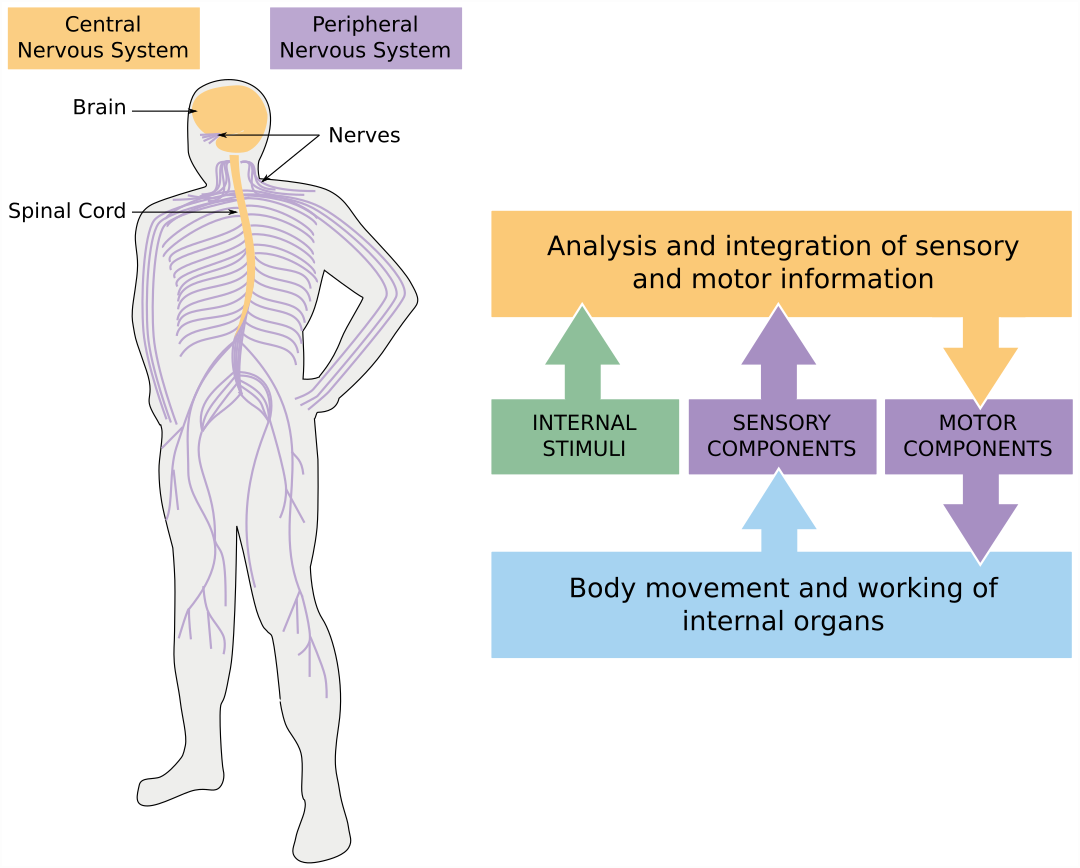
\includegraphics[width=0.49\textwidth]{2.background/neuroanatomy/img/pns_and_cns.png}
    \caption{The two anatomical divisions of the nervous system and their functional relationship.
             Left. Simplified representation of the CNS and PNS in the human.
             Right. Diagram representing the interaction between both subnetworks. Internal and external stimuli gathered by the PNS are proccessed by the CNS, which decides how to respond.
             WE STOLE THIS IMAGE}
    \label{fig:cns_and_pns}
\end{figure}  


In this thesis we will focus only on the brain, which constitutes the upper part of the central nervous system and regulates all human activity.

\section{A Microscopic View of the Human Brain}
\cite{Waehnert2014}

At a microscopical view, the human brain is composed by cells that can be divided in two broad categories: nerve cells (or neurons), and supporting cells called neuroglia (or simply glia).
Nerve cells are discrete entities that communicate with one another by means of specialized contacts that Sherrington called “synapses.” [SHERRINGTON]
Supporting cells, in contrast, are not capable of electrical signaling; nevertheless, they have several essential functions in the developing and adult brain.
The human brain possess on average 86.06 +/- 8.12 billion neurons and 84.61 +/- 2.17 billion nonneuronal cells, making it a linearly scaled-up primate brain in its cellular composition.
In terms of distribution, 80\% of the neurons are present in the cerebellum, meanwhile only 19\% of the nonneural are present there.

\subsection{Neurons}

The basic cellular organization of neurons resembles that of other cells; however, they are clearly distinguished by specialization for intercellular communication.
This attribute is apparent in their overall morphology, in the specific organization of their membrane components for electrical signaling, and in the structural intricacies of the contacts between neurons.
The most obvious sign of neuronal specialization for communication via electrical signaling is the extensive branching of neurons.
The most salient aspect of this branching for typical nerve cells is the elaborate arborization of dendrites that arise from the neuronal cell body (also called dendritic branches or dendritic processes).
The spectrum of neuronal geometries ranges from a small minority of cells that lack dendrites altogether to neurons with dendritic arborizations that rival the complexity of a mature tree (see Figure 1.2).
The number of inputs that a particular neuron receives depends on the complexity of its dendritic arbor: nerve cells that lack dendrites are innervated by (thus, receive electrical signals from) just one or a few other nerve cells, whereas those with increasingly elaborate dendrites are innervated by a commensurately larger number of other neurons.
Nerve cells that carry information toward the brain or spinal cord (or farther centrally within the spinal cord and brain) are called afferent neurons; nerve cells that carry information away from the brain or spinal cord (or away from the circuit in question) are called efferent neurons. Interneurons or local circuit neurons only participate in the local aspects of a circuit, based on the short distances over which their axons extend. These three functional classes—afferent neu- rons, efferent neurons, and interneuronsi are the basic constituents of all neural circuits.

Cortical neurons can be divided in two major types: granule neurons and pyramidal neurons \cite{Johns}.

Granule cells are star-shaped neurons with a typical diameter of less than 20$\mu$m.
They are multipolar neurons, this is, neurons that posses a single axon and many dendrites.
Granule cells are either excitatory, which means they release the neurotransmitter glutamate to send signals to other cells, or inhibitory \cite{Bekkers2011}, which means they release gamma-Aminobutryc acid to reduce neuronal excitability throughout the nervous system.
Granule neurons mostly have purely ‘intrinsic’ axons - they do not enter white matter and make only short-range, local connections.

Pyramidal neurons have large, pyramid-shape bodies that range from 20-120$\mu$m.
Pyramidal neurons are multipolar and excitatory neurons, and they comprise about two-thirds of all neurons in the mammalian cerebral cortex.
On top of their numerical dominance, pyramidal neurons are also 'projection neurons', meaning that they axons are often 'extrinsic' - they make long connections through the white matter.

Another important type of neurons to this thesis are the spindle neurons \cite{Johns}.
Spindle neurons, also called von Economo neurons (VENs), are a specific clfass of neurons that are characterized by a large spindle-shaped soma (or body), gradually tapering into a single apical axon in one direction, with only a single dendrite facing opposite.
VENs emerged within the last decade as having a potentially major role in self-awareness and social cognition in humans \cite{Evrard2012}.

\subsection{Neuroglial}
Neuroglial cells are quite different from nerve cells.
The major distinction is that glia do not participate directly in synaptic interactions and electrical signaling, although their supportive functions help define synaptic contacts and maintain the signaling abilities of neurons.
Although glial cells also have complex processes extending from their cell bodies, these are generally less prominent than neuronal branches, and do not serve the same purposes as axons and dendrites (Figure 1.5).
The term glia (from the Greek word γλοιός meaning “glue”) reflects the nineteenth-century presumption that these cells held the nervous system together in some way.
The word has survived, despite the lack of any evidence that binding nerve cells together is among the many functions of glial cells.
Glial roles that are well-established include maintaining the ionic milieu of nerve cells, modulating the rate of nerve signal propagation, modulating synaptic action by controlling the uptake of neurotransmitters at or near the synaptic cleft, providing a scaffold for some aspects of neural development, and aiding in (or impeding, in some instances) recovery from neural injury.

\subsection{Neuronal Organization: Cortical Layers}

[JOHNS CLINICAL NEUROSCIENCE]
More than 90\% of the cerebral cortex has a characteristic six-layered structure that appeared with the evolution of the mammalian brain (Fig. 5.2).
For this reason it is referred to as neocortex.
Although the same six layers can be identified in all neocortical regions at some stage of development, they are not always present in the mature brain.
The layer structure varies spa- tially in regard to cell organization (cytoarchitecture) and myelination (myeloarchitecture), de fi ning distinct cortical areas which are likely to perform different functions.\cite{Waehnert2014, Bok1929}
Some regions of the cortex are referred to as agranular cortex since they have lost their internal granule cell layer.


\section{A Macroscopic view of the Human Brain}

Neurons never function in isolation; they are organized into circuits or structures that process specific kinds of information.
The brain comprises a diverse collection of these neural structures, each with a distinctive shape and an intricate internal architecture.
Brain tissue can be divided into grey and white matter.
Grey matter is composed mainly of neuronal cell bodies, dendrites and synapses.
It is sharply demarcated from the adjacent white matter, which is made up mostly of tightly packed axons travelling to other parts of the nervous system.
The pale colour of white matter is due to the lipid-rich myelin sheath that surrounds axons and enhances their conduction velocity (see Fig. 1.9; see also Chs 5, 6).

\subsection{Anatomy of the Gray Matter}

The cerebral cortex is the most important structure of the gray matter and plays a major role in cognitive functions.
It is a layered sheet of tissue, 2–3 millimetres thick, highly convoluted.
It's hypothesized that the mechanical tension created by neuronal connections, working against internally generated hydrostatic pressure, is a major driving force of these folds \cite{VanEssen1997}.
These convolutions allow a large surface area to fit within the available cranial volume.
In particular, the human cerebral cortex attains a surface area of about 1600 $cm^2$, nearly three times what it would be in the absence of convolutions 1, 2.
This folding process creates grooves on the surface of the brain called sulci and ridges called gyri.


The cerebral cortex is divided in two hemispheres by a prominent central fissure.
The hemispheres are characterized by the gyri (singular, gyrus) or crests of folded cortical tissue, and sulci (singular, sulcus) the grooves that divide gyri from one another.
Although gyral and sulcal patterns vary from individual to individual, there are some fairly consistent landmarks, particularly the: central sulcus; lateral sulcus; parieto-occipital notch and pre-occipital notch.
These landmarks help divide the hemispheres into four lobes: occipital, temporal, parietal, and frontal.
Hidden from surface view is the insular lobe.

Other structures made of gray matter are the subcortical structures, named like this because they are in the white matter.
Examples of them are the Thalamus, brainstem or hippocampus.

\subsection{Anatomy of the White Matter}
[CATANI]
Axons in the central nervous system are gathered into tracts that are more or less analogous to nerves in the periphery.
Most of the cerebral fibers forming the white matter connect distant regions within the cortex.
There are some fibers that, although being located in the cerbal hemispheres do not connect the cortex, but only subcortical structures.
Fibres group together to form bundles of different diameter and several bundles form larger pathways called fasciculi, or tracts.
Some of these major bundles are well defined in the modern neuronanatomy.

Examples of major bundles in the human brain are the Corpus Callosum, the Internal Capusule and the Superior Longitudinal Fasciculus.
The Corpus Callosum is the largest tract of the human brain, composed of some 200–300 million myelinated axons it connects both hemispheres, allowing to transfer information from one to another.
The internal capsule contain ascending fibres mainly from the thalamus to the cortex, and descending fibres from the cortex to subcortical structures, and the spinal cord.
This complex projection system conveys sensorial information to the cortex and controls movement.
The Inferior Longitudinal Fasciculus is a tract with long and short fibres connecting the occipital and temporal lobes.
Its involved in visual and language functions.


\subsection{Neuroanatomical Naming Conventions}

Brain's anatomy is described from its surface, by means of orthogonal sections and tract dissections [Catani's book].

The surface of the brain can be viewed from the side (lateral view), the middle (medial view), the front (anterior or frontal view), and the back (posterior or occipital view)~\ref{fig:anatomy_terminology}
The same terminology is used to indicate different regions of the brain surface (e.g. dorso-lateral prefrontral cortex).


Sectional neuroanatomy describes the relationship between cortical and subcortical structures, most commonly visualized along orthogonal axial, coronal, and sagital planes~\ref{fig:anatomy_terminology}.
In radiological convention, the axial slices are viewed from the feet towards the head. The coronal planes are conventionally oriented with the left side of the brain on the right side of the page (frontal view).
Finally, the sagittal plane divides the brain into two hemispheres.

Connectional neuroanatomy delineates the origin, course, and termination of connecting pathways~\ref{fig:anatomy_terminology}.
The tracts are classified according to their course and terminal projections.
Commisural pathways run along a horizontal axis and connect the two hemispheres.
The majority of the projection pathways have a perpendicular course along a dorso-ventral (descending) or ventro-dorsal (ascending) axis and connect the cerebral cortex to subcortical nuclei, cerebellum, and the spinal cord.
The association tracts run longitudinal along an antero-posterior axis and connect cortical areas within the same hemisphere.

\begin{figure*}[h!]                                                                                                                    
    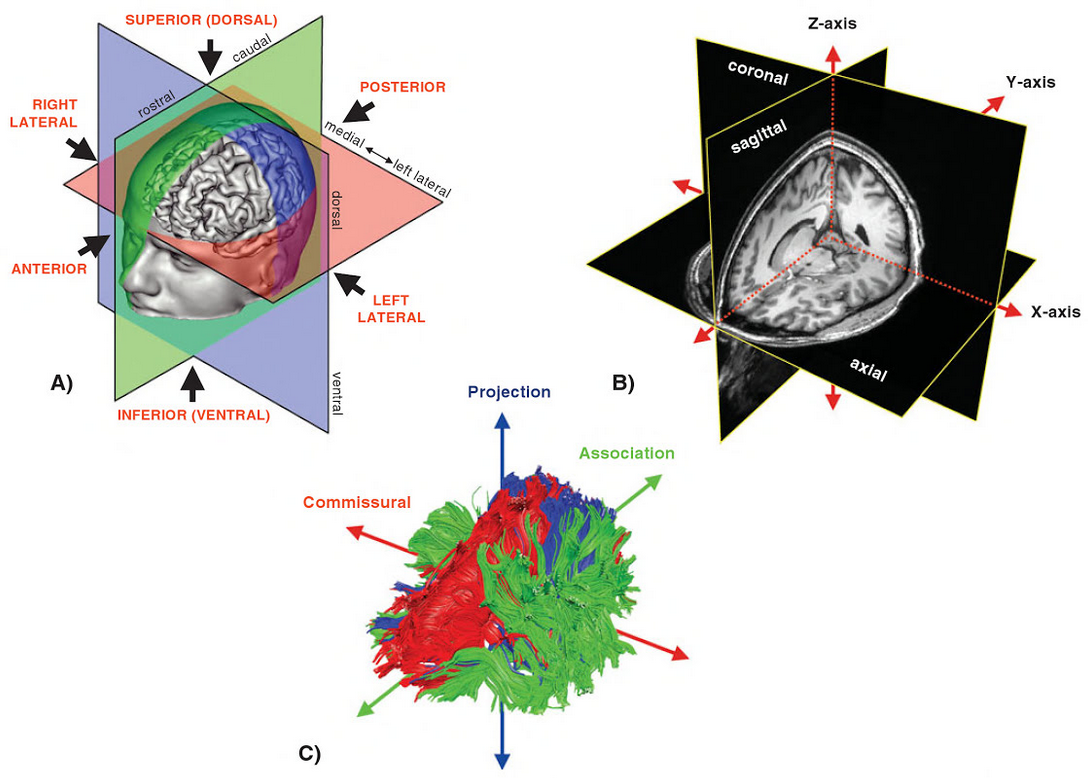
\includegraphics[width=\textwidth]{2.background/neuroanatomy/img/terminology.png}
    \caption{Terms commonly used to describe the orientation of the brain in surface (A), sectional (B) and connectional anatomy (C) representations.}
    \label{fig:anatomy_terminology}
\end{figure*}

This rudimentary description of some prominent anatomical landmarks
provides a framework for understanding how neurons resident in a number of widely distributed and distinct brain structures communicate with one another to define neural systems dedicated to encoding, processing and relaying specific sorts of information about aspects of the organism’s envi- ronment, and then initiating and coordinating appropriate behavioral responses.

\section{Cytoarchitectonics}
The cerebral cortex is divided into more than fifty regions based on its cellular composition under the microscope.
The most known and frequently cited cythoarchitectural organization is that of Brodmann [BROADMANN].
[Figure of broadman around here]

\section{Brain Function}
[CLINICAL NEUROSCIENCE]

While the cerebral hemispheres are specialized to carry out particular cognitive functions, which are said to be lateralized, each lobe has a main role.
Here we present the general function of each lobe, while introducing some of their most important functional subdivisions.
Once again, we do not give a lot of details, but only focus in which is most important for this thesis.

\subsection{Frontal Lobe}
The frontal lobe, responsible for motor functions, speech production, personality, insight and foresight;

The precentral gyrus, immediately anterior to the central sulcus contains an inverted, point-to-point map of the motor functions of the opposite half of the body.
This are is called primary motor cortex (BA 4).
It was discovered by our dear friend Penfield.
The representation of each body part in the motor strip is proportional to the precision of movement control. This means that the areas for the hands, face and tongue are disproportionately large [fig].
The region in front of the motor strip is the lateral premotor area (BA 6) but it does not correspond to any particular gyral or sulcal boundaries.
The premotor cortex also contains an inverted body map and is concerned with preparation and execution of movement sequences in response to external stimuli (as catching a ball, rather than throwing one).
More anteriorly, the frontal eye field (BA 8) is a cortical centre for attention and gaze which directs both eyes towards the contralateral visual field.
The large portion of the frontal lobe anterior to the motor and premotor areas is the prefrontal cortex and is involved in personality, behaviour, language and intellect.
Its mainly concerned with organizing and planning behaviour in pursuit of short-, medium- and long-term goals.
It also has a predominantly inhibitory role, preventing inappropriate behaviour [MARIANO SIGMAN]

Broca’s area is involved in the expressive aspects of spoken and written language (production of sentences constrained by the rules of grammar and syntax). 
It corresponds to the opercular and triangular parts of the inferior frontal gyrus (BA 44 and 45) [FIGURE LANGUAGE]


\subsection{Parietal Lobe}
The parietal lobe, responsible for language comprehension, spatial orientation and perception, and somatic senses, such as touch and temperature.
The postcentral gyrus is immediately posterior to the central sulcus, behind and parallel to the motor strip.
It corresponds to the primary somatosensory cortex (BA 3, 1 and 2).
The sensory strip contains an inverted map of the opposite side of the body that mirrors that of the motor strip, but the relative proportions of the body parts reflect the degree of tactile sensitivity.

\subsection{Occipital Lobe}
The occipital lobe is concerned entirely with visual processing and association.
The retina contains a point-to-point (retinotopic) representation of the visual fields which is maintained throughout the central visual pathways.
Posterior to the chiasm, the optic tracts continue on each side to the lateral geniculate nucleus (LGN) of the thalamus where they synapse.
Thalamocortical neurons then project to the primary visual cortex, via the optic radiations.
The central visual pathways are crossed. This means that the right visual field is represented in the left occipital lobe and vice versa.
[Clinical neuroscience picture 3.7]
The primary visual cortex is highly specialized for processing information about static and moving objects and is excellent in pattern recognition

\subsection{Temporal Lobe}
The temporal lobe is involved in hearing, speech comprehension and visual recognition.
The auditory cortex contains a tonotopic map that represents the audible frequency spectrum (low frequencies laterally, high frequencies medially).
the fusiform gyrus (Latin: fusiform, shaped like a spindle) receives projections from the occipital lobe (part of the ‘what pathway’) and appears to be involved in the recognition of complex visual patterns.
It contributes to reading (in the language-dominant hemisphere) and face recognition (in the non-dominant hemisphere).

Wernicke’s area (pronounced: VER-nikker) corresponds to the posterior third of the superior temporal gyrus and is part of the auditory association cortex [FIGURE LANGUAGE], it's involved in transforming the visual impression of letters (graphemes) into mental representations of speech sounds (phonemes).

\subsection{Insula}

insular stuff


\section{Brain Networks}

The lobes and subcortical structures do not function in isolation, in fact they are heavily connected through the fibre bundles which compose the white matter.

[VINOD]
In his view, the human brain contains at least five major core functional networks: (i) a spatial attention network anchored in posterior parietal cortex and frontal eye fields;
(ii) a language network anchored in Wernicke’s and Broca’s areas; (iii) an explicit memory network anchored in the hippocampal–entorhinal complex and inferior parietal cor- tex; (iv) a face-object recognition network anchored in
midtemporal and temporopolar cortices; and (v) a working memory-executive function network anchored in prefron- tal and inferior parietal cortices. 

\bibliography{bibliography}
